\documentclass[pdf]{beamer}
\mode<presentation>{
	\usetheme{Copenhagen}
	\usecolortheme{seahorse}
}


%% Language and font encodings
\usepackage[frenchb]{babel}

\usepackage[utf8]{inputenc}
\usepackage[T1]{fontenc}

\usepackage{verbatim}
\usepackage{enumitem}
\usepackage{hyperref}

% bibliography package            
\usepackage[backend = biber, style = numeric]{biblatex}   
\addbibresource{references.bib}            

% pour les images
\usepackage{graphicx}
\usepackage{caption} 
\usepackage{float} 
\usepackage{wrapfig}

\usepackage[colorinlistoftodos]{todonotes}
\usepackage{multimedia}

\title[]{Notation symbolique de flux de contrôle musicaux et multimédia}
\institute[]{Faculté des sciences - Université de Montpellier}
\author[]{Vincent Iampietro\\[2ex] {\small \textit{Encadrants:} \\ Jean Bresson \\ Rama Gottfried}}

\AtBeginSection[]
{
	\begin{frame}[plain]{Sommaire}
	\tableofcontents[currentsection]
	\end{frame}
}

\beamertemplatenavigationsymbolsempty

\begin{document}

\begin{frame}[plain]
	\titlepage
\end{frame}

\begin{frame}[plain]{Sommaire}
	\tableofcontents
\end{frame}

%%%%%%%%%%%%%%%%%%%%%%%%%%%%%%%%%%%%%%%%%%%%%%%%%
%%  DE LA NOTATION DE LA MUSIQUE CONTEMPORAINE %%
%%%%%%%%%%%%%%%%%%%%%%%%%%%%%%%%%%%%%%%%%%%%%%%%%
\section[De la notation]{De la notation de la musique contemporaine}

\subsection[Notation traditionnelle]{La notation traditionnelle occidentale}
\begin{frame}{Exemple de pièce de l'époque romantique}
\begin{center}
\textbf{Quatuor à cordes No.14 (\textit{La Jeune Fille et la Mort}), F. P. Schubert, 1824}\\
\movie[]{\fbox{play}}{./medias/ChopinMazurkaOp17No4.aiff}
\end{center}
\end{frame}

\begin{frame}
	\begin{figure}
		\centering
		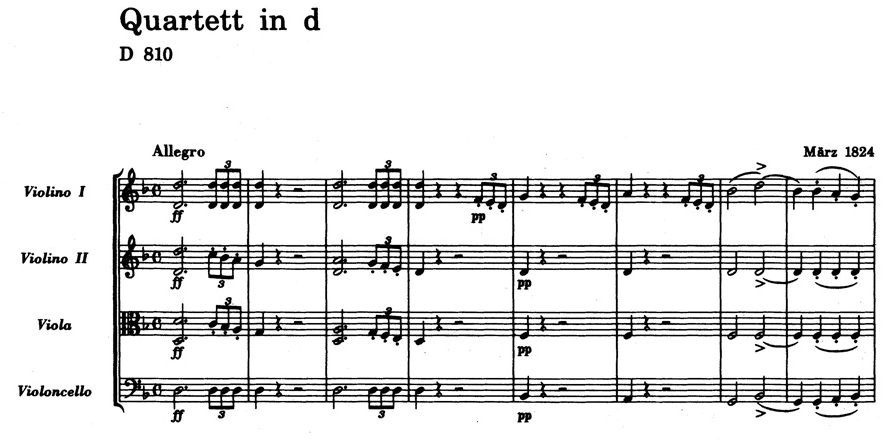
\includegraphics[keepaspectratio=true, width=\textwidth]{./medias/deathAndTheMaiden_extract1.jpg}
		\caption{Extrait de \textit{La jeune fille et la mort}, Franz P. Schubert}
	\end{figure}
\end{frame}

\begin{frame}{Noter la musique}
\begin{figure}
	\centering
	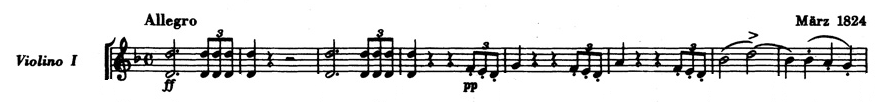
\includegraphics[keepaspectratio=true, width=\textwidth]{./medias/deathAndTheMaiden_extract2.jpg}
\end{figure}
\begin{block}{Le rôle de la partition} 
\begin{itemize}[label={$\square$}]
	\item Un espace de travail pour le compositeur
	\item Médium de partage, de communication
\end{itemize}
\end{block}
\begin{block}{Un système unifié (\textit{Common Western Music Notation})}
\begin{itemize}[label={$\square$}]
	\item Système d'écriture basé sur le symbole		
	\item La portée comme structure centrale
	\item Description de la hauteur, la durée des sons
\end{itemize}
\end{block}

\end{frame}

\subsection{La musique contemporaine}
\begin{frame}{Qu'est-ce que la musique contemporaine}

\begin{block}{Définition}
Ensemble des mouvements de musique savante apparus après la seconde guerre mondiale. La musique savante [...] désigne des traditions musicales impliquant des considérations structurelles et théoriques avancées.
\end{block}

\begin{block}{De nouvelles pratiques}
\begin{itemize}[label={$\square$}]
	\item Utilisation de l'électronique/informatique
	\item Modification du rapport à l'instrument
	\item Modification du rapport au temps
\end{itemize}
\end{block}		

\end{frame}

\begin{frame}{Exemple de pièce de l'époque romantique}
\begin{center}
\textbf{\textit{Mikrophonie I}, K. Stockhausen, 1964}\\
\movie[]{\fbox{play}}{./medias/ChopinMazurkaOp17No4.aiff}
\end{center}
\end{frame}

%%%%%%%%%%%%%%%%%%%%%%%%%%
%%  LE PROJET SYMBOLIST %%
%%%%%%%%%%%%%%%%%%%%%%%%%%
\section[Symbolist]{Le projet symbolist}

\begin{frame}{Présentation du projet}
Slide on the symbolist project.
\end{frame}

%%%%%%%%%%%%%%%%%%%%%%%%%%%%%%%%%%
%% VERS UNE NOTATION EXECUTABLE %%
%%%%%%%%%%%%%%%%%%%%%%%%%%%%%%%%%%
\section[Notation exécutable]{Vers une notation exécutable}

\end{document}
